\documentclass{article}
\usepackage[letterpaper, total={6.5in, 9in}]{geometry}
\usepackage{graphicx} % Required for inserting images
\usepackage{hyperref}
\usepackage[simplified]{pgf-umlcd}
\usepackage{pdflscape}
% \usepackage{emoji}  % LuaLaTeX
% \setemojifont{TwemojiMozilla}

\title{Processing Relay Chat -- PRC}
\author{David Chen -- Team PLA (Pretty Lazy Acronym)}
\date{Period 6}

\begin{document}

\maketitle

\section{Description}
Processing Relay Chat (PRC) encompasses a client program, server program, and protocol for instant messaging over the network. To accomplish this in Processing PRC the \href{https://processing.org/reference/libraries/net/index.html}{Network} library.\\
PRC will include the following minimum features:
\begin{itemize}
    \item Ephemeral plaintext (UTF-8) messaging
    \item IRC-like channels with descriptions
    \item Usernames with deterministic colors
    \item Message timestamps
    \item Light and Dark modes for interface display
\end{itemize}

Optionally, PRC extensions may include (to be implemented after core functionality is complete):
\begin{itemize}
    \item A slash command framework for advanced user interaction
    \item Image embedding, including animated GIFs
    \item Clickable links
    \item File sharing functionality
    \item Chat log export
    \item Simple games embedded in the chat window (Tic-Tac-Toe, Checkers, etc.)
    \item Additional themes for the interface (\href{https://draculatheme.com/}{Dracula}, \href{https://catppuccin.com/}{Catppuccin}, \href{https://www.nordtheme.com/}{Nord}, etc.)
    \item IRC bridging/client-mode compatibility (highly ambitious)
\end{itemize}

%\begin{landscape}
\section{UML Diagram}

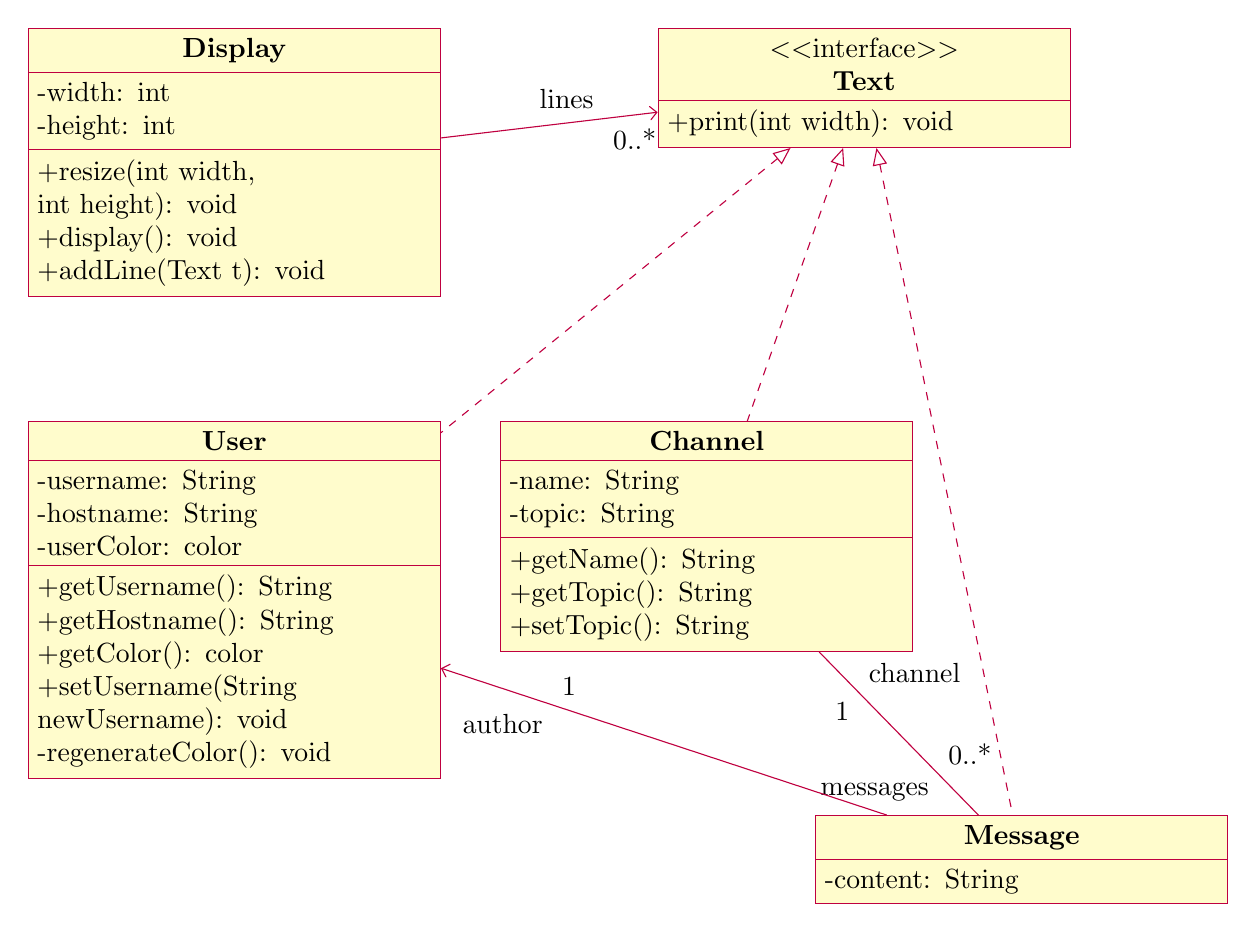
\begin{tikzpicture}
    \begin{class}{Display}{0,0}
        \attribute{-width: int}
        \attribute{-height: int}
        \operation{+resize(int width, int height): void}
        \operation{+display(): void}
        \operation{+addLine(Text t): void}
    \end{class}
    \begin{interface}{Text}{8,0}
        \operation{+print(int width): void}
    \end{interface}
    \begin{class}{User}{0,-5}
        \implement{Text}
        \attribute{-username: String}
        \attribute{-hostname: String}
        \attribute{-userColor: color}
        \operation{+getUsername(): String}
        \operation{+getHostname(): String}
        \operation{+getColor(): color}
        \operation{+setUsername(String newUsername): void}
        \operation{-regenerateColor(): void}
    \end{class}
    \begin{class}{Channel}{6,-5}
        \implement{Text}
        \attribute{-name: String}
        \attribute{-topic: String}
        \operation{+getName(): String}
        \operation{+getTopic(): String}
        \operation{+setTopic(): String}
    \end{class}
    \begin{class}{Message}{10,-10}
        \implement{Text}
        \attribute{-content: String}
    \end{class}
    \unidirectionalAssociation{Display}{lines}{0..*}{Text}
    \association{Channel}{channel}{1}{Message}{0..*}{messages}
    \unidirectionalAssociation{Message}{author}{1}{User}
\end{tikzpicture}\\
(This diagram is getting way too complicated, splitting parts off for now...)

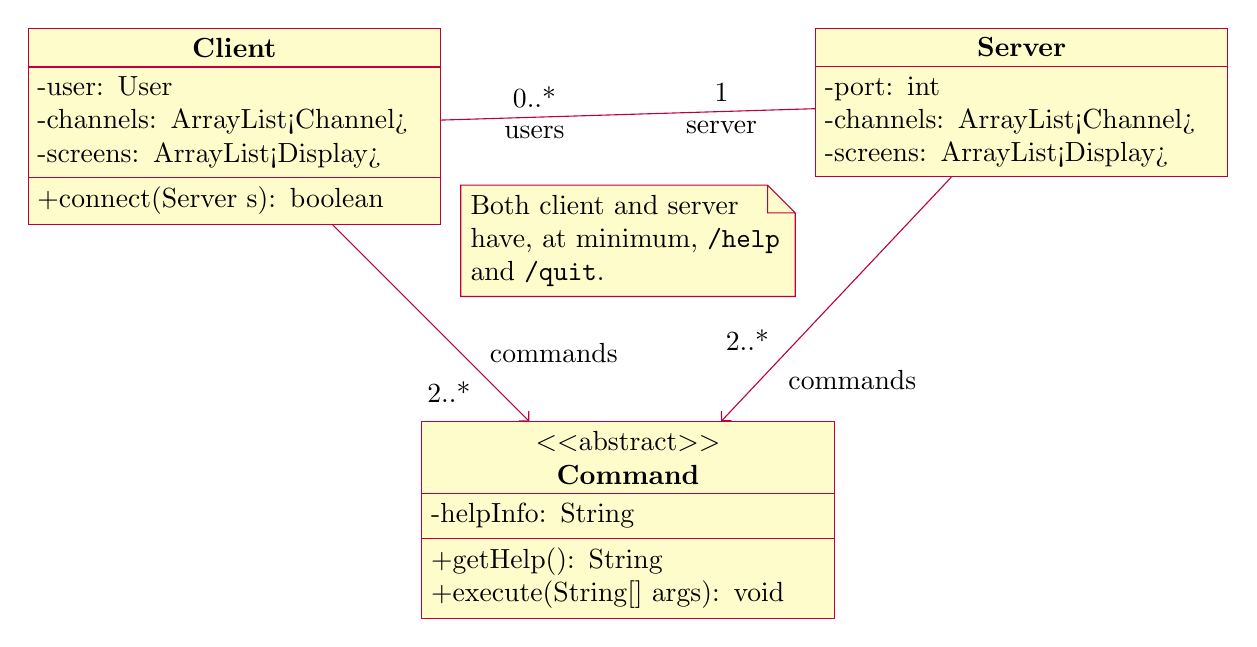
\begin{tikzpicture}
    \begin{class}{Client}{0, 0}
        \attribute{-user: User}
        \attribute{-channels: ArrayList<Channel>}
        \attribute{-screens: ArrayList<Display>}
        \operation{+connect(Server s): boolean}
    \end{class}
    \begin{class}{Server}{10,0}
        \attribute{-port: int}
        \attribute{-channels: ArrayList<Channel>}
        \attribute{-screens: ArrayList<Display>}
    \end{class}
    \begin{abstractclass}{Command}{5,-5}
        \attribute{-helpInfo: String}
        \operation{+getHelp(): String}
        \operation{+execute(String[] args): void}
    \end{abstractclass}
    \association{Server}{server}{1}{Client}{users}{0..*}
    \unidirectionalAssociation{Client}{commands}{2..*}{Command}
    \unidirectionalAssociation{Server}{commands}{2..*}{Command}
    \umlnote[draw] at (5, -2) (commands-note) {Both client and server have, at minimum, \verb|/help| and \verb|/quit|.};
\end{tikzpicture}

%\end{landscape}
\newpage

\section{Manual}
The main Processing program will serve as a launcher, allowing the user to select from server or client modes (or, perhaps, both simultaneously, analogous to LAN multiplayer in video games).

\subsection{Server Mode}
The user will be able to select a TCP port for the server to broadcast on.

The program will then display a log of server interactions (user connections, messages, disconnections). The user can quit the program using \verb|/quit|.

\subsection{Client Mode}
The user will then enter a server address/port to connect to. On successful connection, the user can register a username, which the server will check for uniqueness. If the username is rejected, the user is prompted to enter another username.

The client will then be offered a list of channel names (and their corresponding topics). The client can choose to connect to a channel, upon which they will be put into a chat window view.


\subsubsection{Chat Window}
The main chat window will display messages, usernames, and timestamps. Below the chat window, an input will be available for user messages/commands.

\paragraph{Slash Commands}
To join a room, use \verb|/join|. To leave a room, use \verb|/leave.| To quit the client, use \verb|/quit| (aliased to \verb|/q|).

For information on further commands, use \verb|/help|.

\section{Functionality}
The goal for the coming week is to begin the initial framework for PRC; implementing all minimum features described in the specification.

\subsection{Issues}
None... yet.

\section{Log}
\begin{itemize}
    \item 05/20 -- 05/22: Began writing program specifications in \LaTeX.
\end{itemize}

\end{document}
